% Rapport d'analyse des résultats NLI4CT
% Généré à partir des notebooks error_analysis_* et compare_error

\documentclass[11pt,a4paper]{article}
\usepackage[utf8]{inputenc}
\usepackage[T1]{fontenc}
\usepackage[french]{babel}
\usepackage{geometry}
\usepackage{graphicx}
\usepackage{booktabs}
\usepackage{multirow}
\usepackage{float}
\usepackage{hyperref}
\usepackage{xcolor}

\geometry{margin=2.5cm}
\graphicspath{{../compare_figures/}{../Prompt 1/figures/}{../Prompt 2/figures/}{../Fewshot/figures/}}

\title{Rapport d'analyse des résultats \\ NLI4CT : Finetuning vs Few-shot}
\author{Analyse automatique des notebooks}
\date{\today}

\begin{document}
\maketitle
\tableofcontents
\newpage

%=============================================================================
\section{Introduction}
%=============================================================================

Ce rapport synthétise les résultats des analyses d'erreurs réalisées sur le jeu NLI4CT (Natural Language Inference for Clinical Trials), à partir des notebooks suivants :
\begin{itemize}
  \item \texttt{error\_analysis\_prompt1.ipynb} : analyse Prompt 1 (baseline vs finetuné)
  \item \texttt{error\_analysis\_prompt2.ipynb} : analyse Prompt 2 (baseline vs finetuné)
  \item \texttt{error\_analysis\_fewshot\_prompt1.ipynb} : analyse Few-shot Prompt 1
  \item \texttt{compare\_error.ipynb} : comparaison des trois approches (P1 Finetuné, P2 Finetuné, Few-shot)
\end{itemize}

Jeu de test : 500 exemples (gold test). Les métriques sont l’accuracy globale et les répartitions par type (Single / Comparison), par section (Eligibility, Intervention, Results, Adverse Events), et par longueur de prompt.

%=============================================================================
\section{Accuracy globale}
%=============================================================================

\subsection{Comparaison des approches}

\begin{table}[H]
  \centering
  \caption{Accuracy globale (\%).}
  \label{tab:acc-globale}
  \begin{tabular}{lc}
    \toprule
    Approche & Accuracy \\
    \midrule
    P1 Baseline & 65,80\% \\
    P1 Finetuné & 74,20\% \\
    P1 Few-shot & 72,00\% \\
    P2 Baseline & 65,20\% \\
    P2 Finetuné & 71,80\% \\
    \bottomrule
  \end{tabular}
\end{table}

Le finetuning améliore la baseline pour les deux prompts (P1 : +8,4 points, P2 : +6,6 points). Le few-shot (Prompt 1) est entre baseline et finetuné P1 (72\%).

\begin{figure}[H]
  \centering
  
\includegraphics[width=0.95\textwidth]{../compare_figures/01_accuracy_globale.png}
  \caption{Accuracy globale — tous les prompts et Few-shot.}
  \label{fig:acc-globale}
\end{figure}

%=============================================================================
\section{Résultats par type (Single vs Comparison)}
%=============================================================================

D’après \texttt{compare\_error.ipynb}, les accuracy par type sont cohérentes avec la synthèse : Comparison est plus difficile que Single pour tous les modèles.

\begin{table}[H]
  \centering
  \caption{Accuracy par type (Comparison / Single) — valeurs typiques du compare.}
  \label{tab:acc-type}
  \begin{tabular}{lccccc}
    \toprule
    Type & P1 Bl & P1 FT & P2 Bl & P2 FT & P1 FS \\
    \midrule
    Comparison & 62,4\% & 72,0\% & 60,1\% & 67,9\% & 69,7\% \\
    Single & 70,8\% & 76,9\% & 72,0\% & 76,4\% & 74,7\% \\
    \bottomrule
  \end{tabular}
\end{table}

\begin{figure}[H]
  \centering
  
\includegraphics[width=0.95\textwidth]{../compare_figures/02_accuracy_par_type.png}
  \caption{Accuracy par type (Single / Comparison).}
  \label{fig:acc-type}
\end{figure}

%=============================================================================
\section{Résultats par section}
%=============================================================================

Les sections les plus difficiles (nombre d’erreurs) et les meilleures accuracy (finetuné / few-shot) sont résumées ci-dessous.

\subsection{Prompt 1 (finetuné)}
\begin{itemize}
  \item Sections les plus difficiles (nombre d’erreurs) : Eligibility (41), Intervention (36), Results (27).
  \item Meilleures accuracy par section (finetuné) : Adverse Events 79,2\%, Intervention 74,6\%, Results 74,5\%.
  \item Types : Comparison 72,0\%, Single 76,9\%.
\end{itemize}

\subsection{Prompt 2 (finetuné)}
\begin{itemize}
  \item Sections les plus difficiles : Eligibility (45), Intervention (42), Results (28).
  \item Meilleures accuracy par section : Adverse Events 78,3\%, Results 73,6\%, Intervention 70,4\%.
  \item Types : Comparison 67,9\%, Single 76,4\%.
\end{itemize}

\subsection{Few-shot (Prompt 1)}
\begin{itemize}
  \item Sections les plus difficiles : Intervention (44), Eligibility (40), Adverse Events (31).
  \item Meilleures accuracy par section : Results 76,4\%, Adverse Events 74,2\%, Eligibility 69,7\%.
  \item Types : Comparison 69,7\%, Single 74,7\%.
\end{itemize}

\begin{figure}[H]
  \centering
  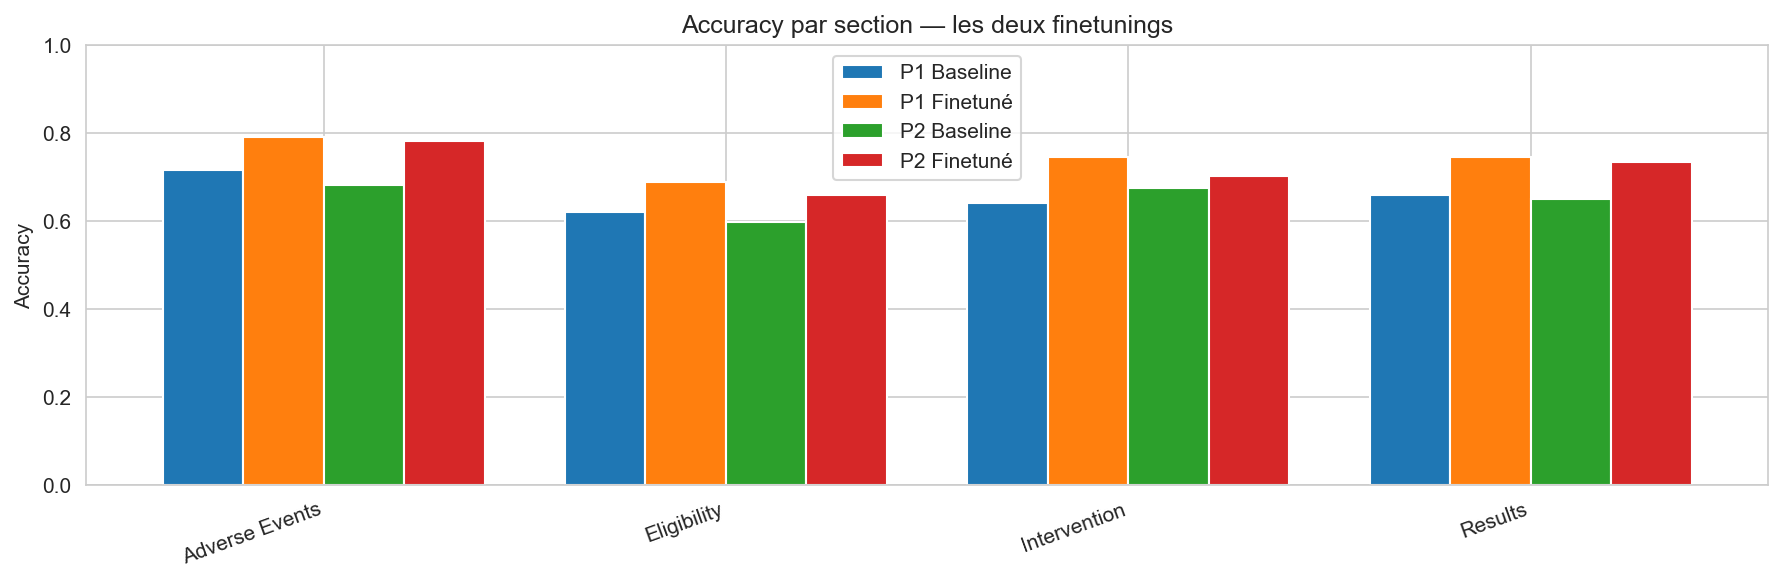
\includegraphics[width=0.95\textwidth]{../compare_figures/03_accuracy_par_section.png}
  \caption{Accuracy par section (toutes approches).}
  \label{fig:acc-section}
\end{figure}

%=============================================================================
\section{Longueur du prompt et performance}
%=============================================================================

Pour les modèles finetunés, les erreurs correspondent en moyenne à des prompts plus longs que les corrects.

\begin{table}[H]
  \centering
  \caption{Longueur moyenne du prompt (caractères).}
  \label{tab:longueur}
  \begin{tabular}{lcc}
    \toprule
    & Longueur (corrects) & Longueur (erreurs) \\
    \midrule
    Prompt 1 (finetuné) & 871 & 1406 \\
    Prompt 2 (finetuné) & 932 & 1420 \\
    Few-shot P1 & 1017 & 988 \\
    \bottomrule
  \end{tabular}
\end{table}

Pour le few-shot, la différence de longueur entre corrects et erreurs est faible (1017 vs 988). Pour le finetuning, les erreurs sont nettement associées à des prompts plus longs.

\begin{figure}[H]
  \centering
  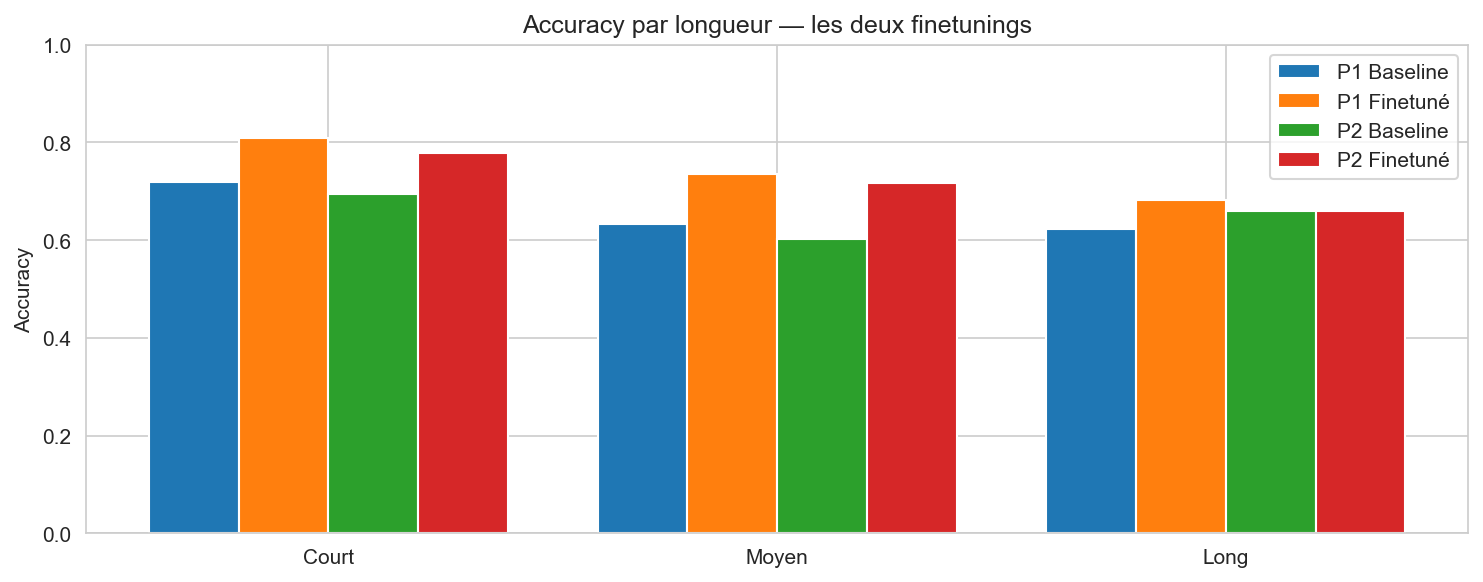
\includegraphics[width=0.95\textwidth]{../compare_figures/04_accuracy_par_longueur.png}
  \caption{Accuracy par bin de longueur (Court / Moyen / Long).}
  \label{fig:acc-longueur}
\end{figure}

%=============================================================================
\section{Régressions et améliorations (Baseline vs Finetuné)}
%=============================================================================

\begin{table}[H]
  \centering
  \caption{Régressions et améliorations par rapport à la baseline.}
  \label{tab:regressions}
  \begin{tabular}{lc}
    \toprule
    & Nombre \\
    \midrule
    P1 Régressions (Bl correct, FT faux) & 60 \\
    P1 Améliorations (Bl faux, FT correct) & 102 \\
    P2 Régressions & 60 \\
    P2 Améliorations & 93 \\
    P1 Few-shot régressions vs P1 FT & 61 \\
    P1 Few-shot améliorations vs P1 FT & 72 \\
    \bottomrule
  \end{tabular}
\end{table}

Le finetuning apporte plus d’améliorations que de régressions pour les deux prompts. Le few-shot (P1) a légèrement plus de régressions que d’améliorations par rapport au P1 Finetuné (61 vs 72).

%=============================================================================
\section{Parties 8, 9 et 10 du notebook compare\_error (cœur de l'analyse)}
%=============================================================================

Les sections 8, 8b, 9, 10 et 10b du notebook \texttt{compare\_error.ipynb} constituent le cœur de la comparaison entre les trois approches (P1 Finetuné, P2 Finetuné, Few-shot) : quand les modèles se trompent ensemble ou quand l'un compense l'autre.

\subsection{Section 8 : Accord / désaccord entre les 3 approches}

Sur les 500 exemples où les trois approches sont évaluées (Few-shot P1 chargé), on forme pour chaque exemple un pattern (P1\_ft, P2\_ft, FS) avec 1 = correct, 0 = erreur. On compte :

\begin{table}[H]
  \centering
  \caption{Patterns d’accord P1 Finetuné / P2 Finetuné / Few-shot (1 = correct, 0 = erreur).}
  \label{tab:patterns}
  \begin{tabular}{llc}
    \toprule
    Pattern & Description & Effectif \\
    \midrule
    111 & Les 3 corrects & 279 \\
    000 & Les 3 en erreur & 59 \\
    110 & P1 ok, P2 ok, FS erreur & 54 \\
    101 & P1 ok, P2 erreur, FS ok & 20 \\
    011 & P1 erreur, P2 ok, FS ok & 17 \\
    100 & P1 ok, P2 erreur, FS erreur & 18 \\
    010 & P1 erreur, P2 ok, FS erreur & 9 \\
    001 & P1 erreur, P2 erreur, FS ok & 44 \\
    \bottomrule
  \end{tabular}
\end{table}

\textbf{Interprétation :} 111 = consensus succès (279, 55,8\%). 000 = échec commun (59, 11,8\%) — cas les plus difficiles. 001 (44) = seul le Few-shot a raison (few-shot compense). 110 (54) = les deux FT ont raison, FS se trompe (finetuning plus fiable). Les autres patterns décrivent les désaccords entre un seul finetuné et le reste.

\begin{figure}[H]
  \centering
  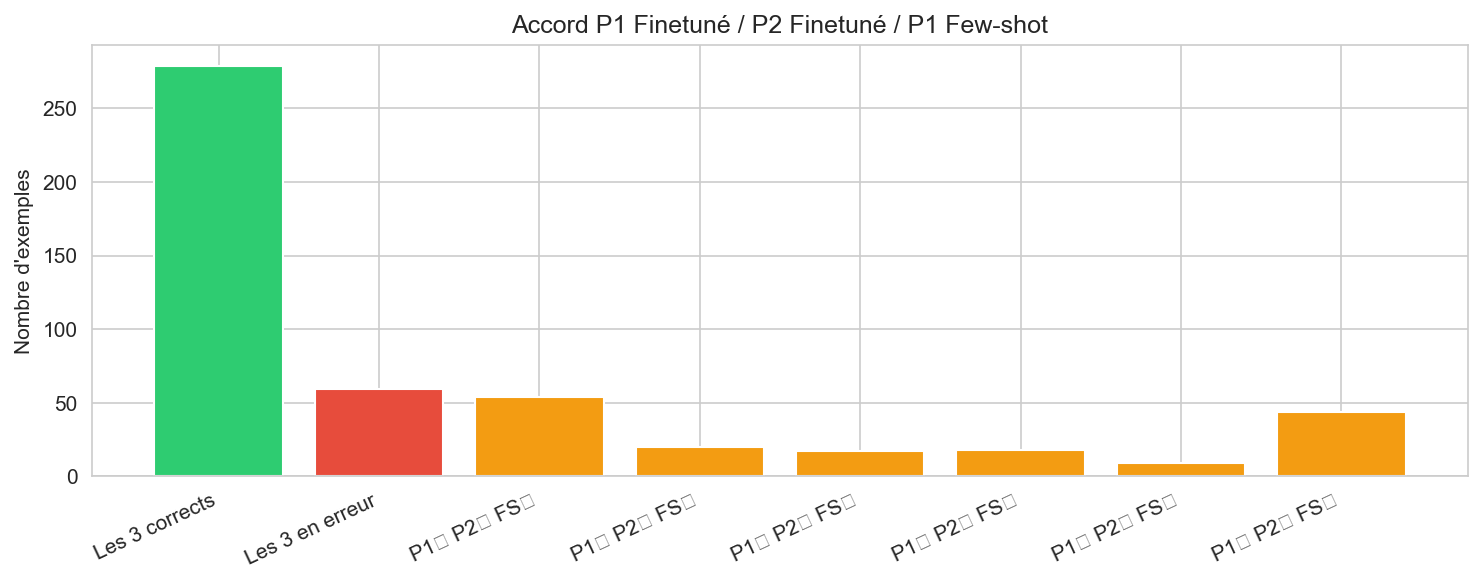
\includegraphics[width=0.95\textwidth]{../compare_figures/08_accord_trois_approches.png}
  \caption{Section 8 : répartition des patterns d’accord entre P1 FT, P2 FT et Few-shot.}
  \label{fig:accord-trois}
\end{figure}

\subsection{Section 8b : Comparaisons deux-à-deux}

Pour chaque paire de modèles on compte : les deux corrects, A correct B faux, A faux B correct, les deux en erreur.

\subsubsection{P1 Finetuné vs P2 Finetuné}

\begin{table}[H]
  \centering
  \caption{Accord P1 Finetuné vs P2 Finetuné.}
  \label{tab:pair-p1p2}
  \begin{tabular}{lc}
    \toprule
    Cas & Effectif \\
    \midrule
    Les deux corrects & 333 \\
    P1 correct, P2 faux & 38 \\
    P1 faux, P2 correct & 26 \\
    Les deux en erreur & 103 \\
    \bottomrule
  \end{tabular}
\end{table}

Les deux modèles finetunés sont d’accord sur 333 + 103 = 436 exemples (87,2\%). P1 FT est seul correct 38 fois, P2 FT 26 fois.

\begin{figure}[H]
  \centering
  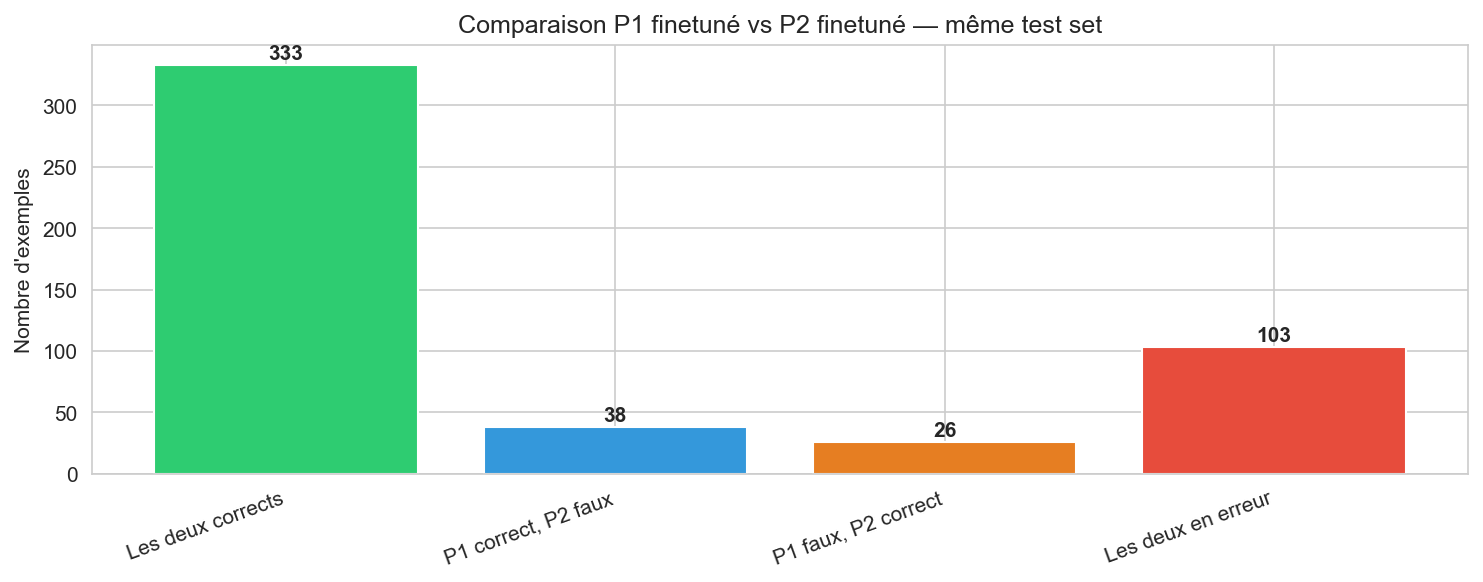
\includegraphics[width=0.85\textwidth]{../compare_figures/08b_compare_ft_p1_vs_p2.png}
  \caption{Comparaison deux-à-deux : P1 Finetuné vs P2 Finetuné.}
  \label{fig:pair-p1p2}
\end{figure}

\subsubsection{P1 Finetuné / P2 Finetuné vs Few-shot}

Les tableaux (P1 vs FS, P2 vs FS) sont affichés dans la section 8b et regroupés dans la figure \ref{fig:accord-pairwise}. On en déduit où le few-shot « sauve » un exemple (correct alors que le FT se trompe) ou où le finetuné est préférable.

\begin{figure}[H]
  \centering
  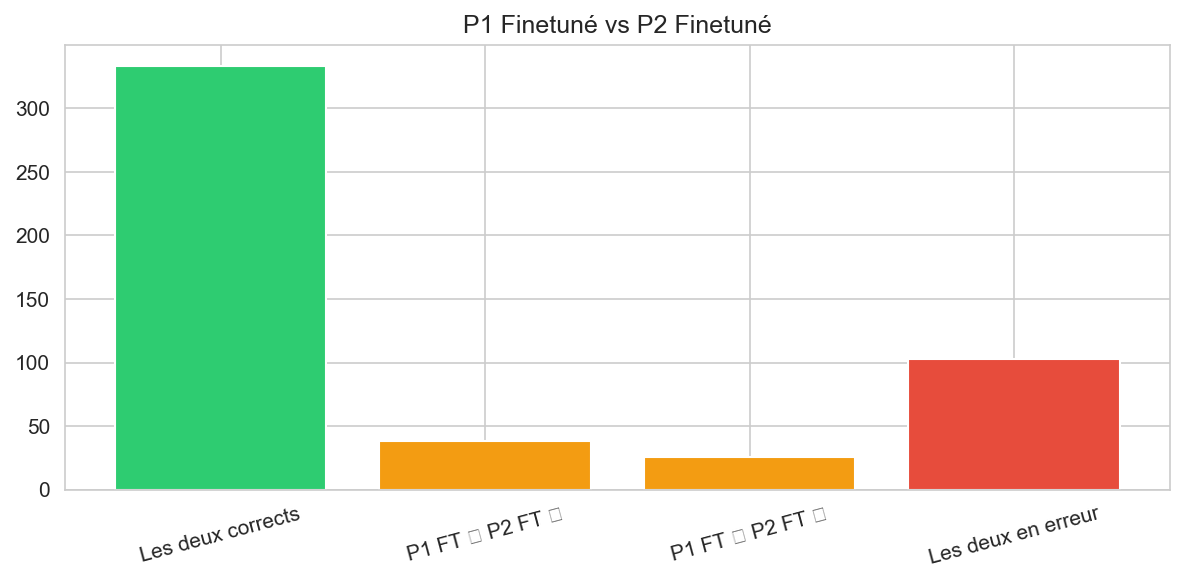
\includegraphics[width=0.95\textwidth]{../compare_figures/08b_pairwise_accord.png}
  \caption{Accord deux-à-deux : P1 vs P2, P1 vs Few-shot, P2 vs Few-shot.}
  \label{fig:accord-pairwise}
\end{figure}

\subsection{Section 9 : Cas où les 3 approches se trompent (ou au moins 2)}

On définit : \textbf{Les 3 en erreur} = pattern 000 (59 exemples). \textbf{Au moins 2 en erreur} = au moins deux des trois se trompent (130 exemples). Le notebook construit \texttt{detail\_3wrong} (index, type, section\_id, true\_label, pred\_P1, pred\_P2, pred\_FS) et l'exporte en \texttt{three\_approaches\_wrong.csv}. La répartition par section des 59 cas (figure \ref{fig:three-wrong}) montre si les échecs communs sont concentrés (p.ex. Eligibility, Intervention). Ces 59 cas sont les plus difficiles ; bons candidats pour rééquilibrage ou revue manuelle.

\begin{table}[H]
  \centering
  \caption{Section 9 : effectifs erreur commune.}
  \label{tab:sec9}
  \begin{tabular}{lc}
    \toprule
    & Effectif \\
    \midrule
    Les 3 en erreur & 59 \\
    Au moins 2 en erreur & 130 \\
    \bottomrule
  \end{tabular}
\end{table}

\subsection{Section 10 : Cas où les 3 approches ont raison}

\textbf{Les 3 corrects} = pattern 111 (279). \textbf{Au moins 2 corrects} = 370. La répartition par section des 279 est en figure \ref{fig:three-ok}.

\begin{table}[H]
  \centering
  \caption{Section 10 : effectifs succès commun.}
  \label{tab:three}
  \begin{tabular}{lc}
    \toprule
    & Effectif \\
    \midrule
    Les 3 corrects & 279 \\
    Au moins 2 corrects & 370 \\
    \bottomrule
  \end{tabular}
\end{table}

\subsection{Section 10b : Exemples pour analyse et répartition par type/section}

Cinq exemples aléatoires (seed 42) pour chacun des trois cas : (1) Les 3 se trompent (000, 59 ex.) ; (2) P1 et P2 FT se trompent, Few-shot a raison (001, 44 ex.) ; (3) Few-shot se trompe, P1 et P2 FT ont raison (110, 54 ex.). Pour \emph{chaque} cas, le notebook affiche la \textbf{répartition par type} et par \textbf{section\_id}. Les 5 exemples affichés pour chaque cas sont les suivants.

\subsubsection*{Cas 1 — Les 3 se trompent (000)}
\textbf{Index 7} (Comparison, Eligibility). Vrai : Contradiction. P1/P2/FS : Entailment. Premise : History of allergic reactions attributed to compounds of similar chemical or biologic composition to mesna or other agents (e.g. sulfur containing drugs\ldots). Hypothesis : Any patients with Documented allergy to cephalosporin or trimethoprim/sulfamethoxazole will not be eligible\ldots

\textbf{Index 97} (Comparison, Eligibility). Vrai : Contradiction. P1/P2/FS : Entailment. Premise : Inclusion Criteria: 18 years or older, Histologically or cytologically confirmed metastatic and/or adva\ldots Hypothesis : Unlike the primary trial, patients must be diagnosed with a mutation in PTEN, BRAF, KRAS, NRAS, PI3KCA, ErbB1, ErbB2\ldots

\textbf{Index 310} (Single, Results). Vrai : Entailment. P1/P2/FS : Contradiction. Premise : Outcome Measurement: Percentage of Participants With Disease Progression or Death; PFS was defined as the time from firs\ldots Hypothesis : the Bevacizumab cohort of the primary trial had a higher incidence of Disease Progression or Death than the Bevacizumab + Capecitabine cohort.

\textbf{Index 150} (Comparison, Eligibility). Vrai : Entailment. P1/P2/FS : Contradiction. Premise : NUT midline carcinoma (ectopic expression of NUT protein, IHC and/or BRD-NUT gene translocation\ldots). Hypothesis : Patients with NUT midline carcinoma or Castrate-resistant prostate cancer, or inflammatory breast ca\ldots

\textbf{Index 384} (Comparison, Eligibility). Vrai : Entailment. P1/P2/FS : Contradiction. Premise : Diagnosis of anemia only due to iron-deficiency; Diagnosis of thalasemic syndromes; Diagnosis of fibromyalgia. Hypothesis : Any cancer patient diagnosed with either fibromyalgia, thalasemic syndromes or anemia cannot be eligible for both the primary trial and the secondary\ldots

\subsubsection*{Cas 2 — P1 et P2 FT se trompent, Few-shot a raison (001)}
\textbf{Index 284} (Comparison, Results). Vrai : Contradiction. P1/P2 : Entailment, FS : Contradiction. Premise : Outcome Measurement: Safety; toxicity graded following NCI Common Toxicity Criteria 2.0. Time frame: 2 ye\ldots Hypothesis : There were more participants in the primary trial than in the secondary trial.

\textbf{Index 421} (Comparison, Eligibility). Vrai : Entailment. P1/P2 : Contradiction, FS : Entailment. Premise : Inclusion Criteria: Adults with histologically or cytologically confirmed breast adenocarcinoma, bone mets, ECOG 0, 1 o\ldots Hypothesis : Patients with histologically confirmed stage 4 breast adenocarcinoma that is either ER positive, PR positive or HER2/neu negative are eligible for bot\ldots

\textbf{Index 21} (Single, Adverse Events). Vrai : Contradiction. P1/P2 : Entailment, FS : Contradiction. Premise : Hypertension 1/8 (12.50\%), Hepatotoxicity 3/8 (37.50\%), Pancreatectomy 1/8 (12.50\%). Hypothesis : in the primary trial there were 10 times the number of Hepatotoxicity cases as there were cases of hypertension and Pancreatectomy.

\textbf{Index 173} (Comparison, Intervention). Vrai : Contradiction. P1/P2 : Entailment, FS : Contradiction. Premise : INTERVENTION 1: Denosumab 120 mg subcutaneously every 4 weeks\ldots INTERVENTION 1: Intraope\ldots Hypothesis : the primary trial requires patients to receive 120 milligrams of denosumab injected subcutaneously every month, the secondary trial does not require i\ldots

\textbf{Index 260} (Comparison, Results). Vrai : Entailment. P1/P2 : Contradiction, FS : Entailment. Premise : Outcome Measurement: Time to Progression (TTP)\ldots Hypothesis : the primary trial reports the Time to Progression in months for a total of 156 patients across the two cohorts, on the other hand, the secondary trial\ldots

\subsubsection*{Cas 3 — Few-shot se trompe, P1 et P2 FT ont raison (110)}
\textbf{Index 65} (Comparison, Adverse Events). Vrai : Contradiction. P1/P2 : Contradiction, FS : Entailment. Premise : Adverse Events 1: Total: 0/104 (0.00\%); Adverse Events 1: Total: 45/128 (35.16\%), Anaemia 3/128 (2.34\%)\ldots Hypothesis : The most common adverse event in the secondary trial was Anaemia, affecting more than 5\% of patients, there were no recorded AEs in the primary trial.

\textbf{Index 5} (Comparison, Adverse Events). Vrai : Entailment. P1/P2 : Entailment, FS : Contradiction. Premise : Adverse Events 1: Total: 0/10 (0.00\%); 0/1699 (0.00\%); 0/2004 (0.00\%). Hypothesis : There are no cases of anorexia, hypothermia or hallucinations recorded in the Aes of the primary trial or the secondary trial.

\textbf{Index 482} (Single, Intervention). Vrai : Contradiction. P1/P2 : Contradiction, FS : Entailment. Premise : INTERVENTION 1: Bisphosphonate IV Q4W; INTERVENTION 2: Denosumab 180 mg Q12W\ldots Hypothesis : The Interventions in the primary trial included different medications but are administered through the same routes.

\textbf{Index 142} (Single, Intervention). Vrai : Entailment. P1/P2 : Entailment, FS : Contradiction. Premise : INTERVENTION 1: SUNITINIB+CAPECITABINE, Sunitinib was administered orally from Day 1 at 37.5 mg/day on a continuous daily dosing schedule\ldots Hypothesis : Sunitinib was administered orally every day, to every patient in the primary trial for the entire duration of the study.

\textbf{Index 441} (Comparison, Adverse Events). Vrai : Entailment. P1/P2 : Entailment, FS : Contradiction. Premise : Diarrhea 7/30 (23.33\%); Diarrhoea 0/6 (0.00\%); Diarrhoea 0/6 (0.00\%). Hypothesis : Diarrhoea was more common for the primary trial participants than the secondary trial participants.

\begin{figure}[H]
  \centering
  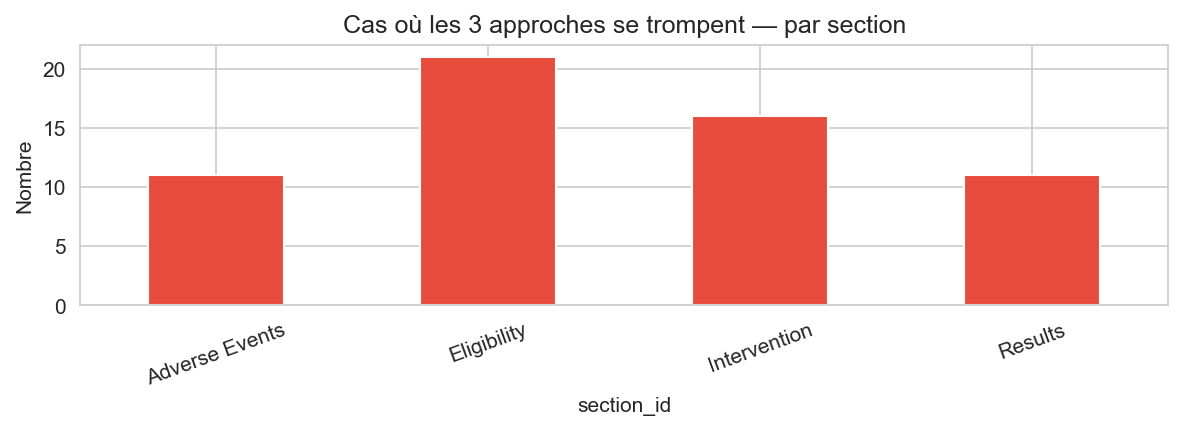
\includegraphics[width=0.85\textwidth]{../compare_figures/09_three_wrong_by_section.png}
  \caption{Section 9 : répartition par section des 59 exemples où les 3 se trompent.}
  \label{fig:three-wrong}
\end{figure}

\begin{figure}[H]
  \centering
  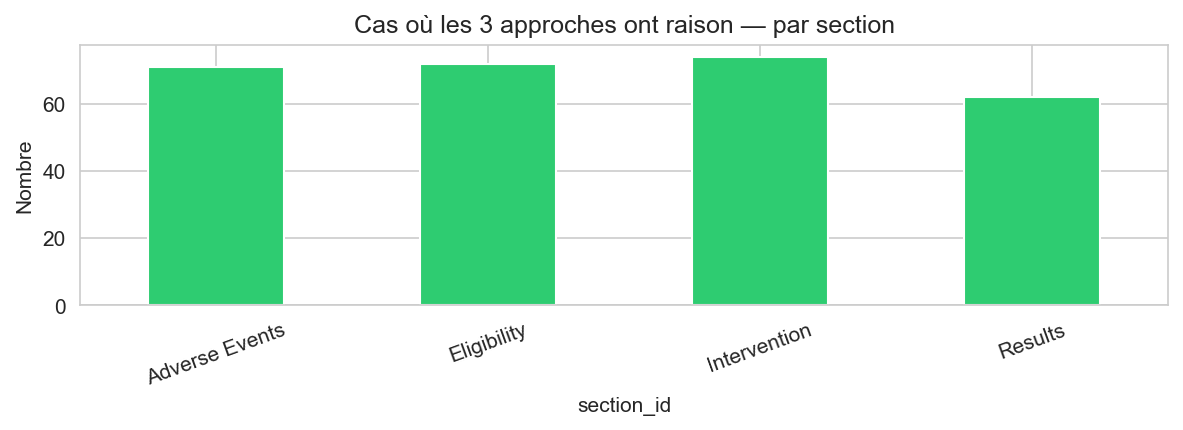
\includegraphics[width=0.85\textwidth]{../compare_figures/10_three_ok_by_section.png}
  \caption{Section 10 : répartition par section des 279 exemples où les 3 ont raison.}
  \label{fig:three-ok}
\end{figure}

Les listes détaillées (index, type, section, labels) sont exportées en CSV : \texttt{compare\_figures/three\_approaches\_wrong.csv} et utilisées pour l’analyse qualitative (exemples 5 par cas : 000, 001, 110) et la répartition par type/section dans la section 10b du notebook.

%=============================================================================
\section{Matrices de confusion et erreurs}
%=============================================================================

Les notebooks produisent des matrices de confusion (vrai label vs prédit) et des graphiques d’erreurs par section. Un point important ressort de ces matrices : la \textbf{baseline prédit majoritairement Contradiction}, alors que le \textbf{finetuning équilibre} les prédictions entre Entailment et Contradiction. Le modèle finetuné apprend ainsi à « prendre des risques » plutôt que de renvoyer systématiquement Contradiction par défaut. Figure de référence :

\begin{figure}[H]
  \centering
  
\includegraphics[width=0.95\textwidth]{../compare_figures/05_erreurs_confusion.png}
  \caption{Exemple de matrices de confusion (erreurs) — comparaison.}
  \label{fig:confusion}
\end{figure}

\begin{figure}[H]
  \centering
  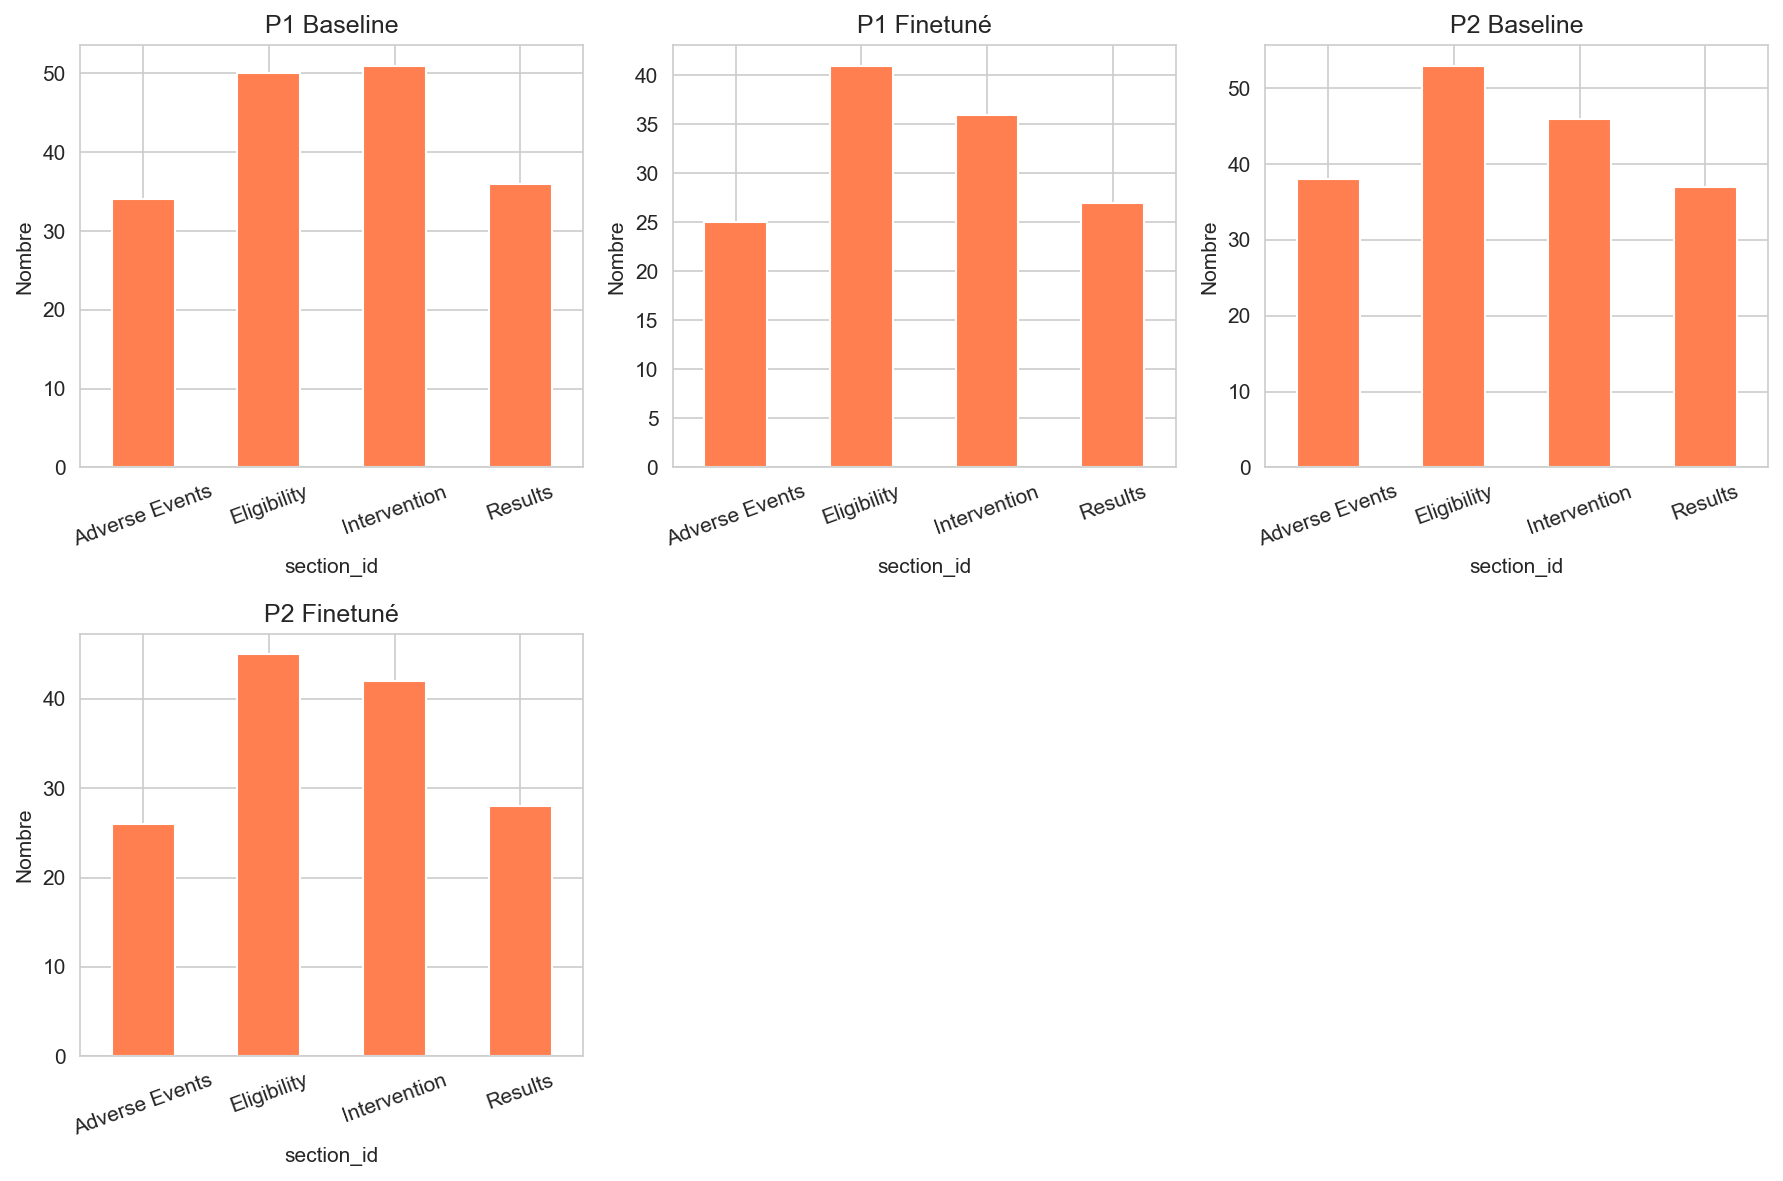
\includegraphics[width=0.95\textwidth]{../compare_figures/06_erreurs_par_section.png}
  \caption{Erreurs par section — comparaison.}
  \label{fig:erreurs-section}
\end{figure}

%=============================================================================
\section{Synthèse par approche}
%=============================================================================

\subsection{Prompt 1 (error\_analysis\_prompt1)}
\begin{itemize}
  \item Accord baseline et finetuné tous deux corrects : 269.
  \item Régressions : 60 ; Améliorations : 102.
  \item Bins longueur (finetuné) : Court 80,8\%, Moyen 73,5\%, Long 68,3\%.
\end{itemize}

\subsection{Prompt 2 (error\_analysis\_prompt2)}
\begin{itemize}
  \item Accord baseline et finetuné tous deux corrects : 266.
  \item Régressions : 60 ; Améliorations : 93.
  \item Bins longueur (finetuné) : Court 77,8\%, Moyen 71,7\%, Long 65,9\%.
\end{itemize}

\subsection{Few-shot Prompt 1 (error\_analysis\_fewshot\_prompt1)}
\begin{itemize}
  \item Nombre de prédictions correctes : 360 / 500 (72\%).
  \item Bins longueur : Court 77,8\%, Moyen 66,3\%, Long 71,9\% (effet longueur moins monotone que pour le finetuning).
\end{itemize}

%=============================================================================
\section{Conclusions}
%=============================================================================

\begin{enumerate}
  \item Le \textbf{finetuning} améliore nettement la baseline pour les deux prompts (P1 74,2\%, P2 71,8\%) et reste supérieur au few-shot (72\%).
  \item Les \textbf{matrices de confusion} montrent que la baseline prédit majoritairement Contradiction, alors que le finetuning équilibre les prédictions : le modèle finetuné apprend à « prendre des risques » et à prédire Entailment lorsque la prémisse supporte l'hypothèse, au lieu de renvoyer systématiquement Contradiction par défaut.
  \item Les tâches \textbf{Comparison} sont plus difficiles que \textbf{Single} pour toutes les approches.
  \item Les sections \textbf{Eligibility} et \textbf{Intervention} concentrent le plus d’erreurs ; \textbf{Adverse Events} et \textbf{Results} ont les meilleures accuracy.
  \item Les \textbf{prompts longs} sont associés à plus d’erreurs pour le finetuning ; l’effet est moins marqué pour le few-shot.
  \item Sur les patterns à trois (P1 FT, P2 FT, Few-shot) : 279 exemples où les 3 ont raison, 59 où les 3 se trompent ; 44 où seul le few-shot a raison (001) et 54 où seul le few-shot a tort (110). Une analyse qualitative (section 10b de \texttt{compare\_error.ipynb}) et la répartition par type/section permettent d’interpréter ces cas.
  \item Les exports (CSV, figures) sont dans \texttt{results/compare\_figures/}, \texttt{results/Prompt 1/figures/}, \texttt{results/Prompt 2/figures/}, \texttt{results/Fewshot/figures/}.
\end{enumerate}

\end{document}
